\documentclass[conference]{IEEEtran}
\IEEEoverridecommandlockouts
% The preceding line is only needed to identify funding in the first footnote.
\usepackage{cite}
\usepackage{amsmath,amssymb,amsfonts}
\usepackage{algorithmic}
\usepackage{graphicx}
\usepackage{textcomp}
\usepackage{xcolor}
\usepackage{booktabs}
\usepackage{multirow}
\usepackage{url}
\usepackage{tikz}
\usetikzlibrary{positioning,arrows.meta,fit}

\hyphenation{re-con-cil-i-a-tion syn-drome Cas-cade}
\makeatletter
% table rows generated by sim/make_tables.py; the primitive input is
% expandable and therefore safe immediately before \bottomrule
\newcommand{\tablerows}[1]{\@@input #1 }
\makeatother

\begin{document}

\title{LUCID-BB84: Syndrome-Lookup Reconciliation for BB84 with Row--Column Iterative Decoding and Block-Level Verification}

\author{\IEEEauthorblockN{[First Author Name]}
\IEEEauthorblockA{\textit{[Department]} \\
\textit{[Institution]}\\
{[City], [Country]} \\
{[e-mail address]}}
\and
\IEEEauthorblockN{Balasubramanian TBR}
\IEEEauthorblockA{\textit{[Department]} \\
\textit{[Institution]}\\
{[City], [Country]} \\
{[e-mail address]}}
}

\maketitle

\begin{abstract}
Interactive Cascade reconciliation ties the latency of BB84 post-processing to the round-trip time of the classical channel. LUCID-BB84 replaces it with a one-way extended-Hamming syndrome lookup, a keyed Toeplitz verification tag, Toeplitz privacy amplification and a Cascade fallback, and its register-transfer-level front end verifies a 512-bit frame in 24 clock cycles. Because a block corrects only one error, frames must stay short, and short frames make per-frame verification costly and per-frame privacy amplification infeasible under finite-key statistics. We extend the design in three ways. LUCID-2D arranges each frame as a grid, sends row and column syndromes in the same single message, and decodes by iterating the same lookup along rows and columns entirely on syndromes, with a communication-free stall-resolution step and a one-round second-syndrome fallback. A block-level pipeline keeps only a short routing tag per frame and moves parameter estimation, the correctness tag and privacy amplification to blocks of about one million bits. A zero-leakage estimator recovers the error rate from syndromes that are already public. In a unified simulator that counts every disclosed bit, LUCID-2D reaches 94 to 98 percent of the secret fraction of a belief-propagation LDPC decoder at 0.1 to 0.5 percent error rate in about one round trip, against some 33 round trips for Cascade, and its verified decoder core uses 4 to 13 percent of a 25k-LUT FPGA at 61 to 84 MHz. At 1 percent error rate and above, LDPC remains the better choice.
\end{abstract}

\begin{IEEEkeywords}
quantum key distribution, BB84, information reconciliation, product codes, Hamming code, LDPC, Cascade, privacy amplification, finite-key analysis, FPGA
\end{IEEEkeywords}

\section{Introduction}
Quantum key distribution (QKD) leaves the two parties with correlated but not identical raw keys. Classical post-processing---sifting, parameter estimation, information reconciliation, verification and privacy amplification (PA)---turns them into identical keys about which an eavesdropper knows essentially nothing \cite{bb84,scarani2009,pirandola2020}. Reconciliation dominates both the information disclosed to the eavesdropper and the latency. Cascade \cite{cascade,demystifying} is close to the Shannon limit but interactive, so its latency grows with the number of public-channel round trips. One-way low-density parity-check (LDPC) syndromes \cite{gallager1962,elkouss2009,elkouss2011} need a single message, at the price of an iterative belief-propagation (BP) decoder \cite{mackay1999,kschischang2001}.

LUCID-BB84 takes the opposite extreme and reduces reconciliation to a table lookup. For every small extended-Hamming block \cite{hamming1950}, Alice publishes its short syndrome; Bob corrects single errors by lookup and flags double errors; a keyed Toeplitz tag verifies the frame; and frames that fail are handed to Cascade. The original study showed that this cuts round trips sharply relative to Cascade at low quantum bit error rate (QBER), but that it does not match one-way LDPC on secret-key rate, and that its main remaining argument---small, fixed-latency hardware---was untested.

Three weaknesses of the one-dimensional design limit it. First, a block corrects at most one error, so the probability that a whole frame decodes falls exponentially with frame length and frames must stay short. Second, with short frames a 64-bit tag per frame costs $64/512=12.5$\% of the key, more than the reconciliation itself at 0.1\% QBER. Third, estimating the phase-error rate and performing PA per 512-bit frame cannot yield a positive key once finite-size statistics are included, as the bound used in Section~\ref{sec:block} shows \cite{tomamichel2012}.

This paper keeps the lookup decoder and removes these limits. Its contributions are:
\begin{enumerate}
\item The LUCID front end: a bit-exact golden model, register-transfer-level (RTL) hardware with measured cycle counts, and a comparison with Cascade and one-way LDPC in which every disclosed bit is counted.
\item LUCID-2D, which places each frame on a grid, sends row and column syndromes in one message, and iterates the same lookup along rows and columns. The decoder operates only on syndromes, adds a communication-free stall-resolution step and a one-round second-syndrome fallback, and is verified and synthesized for field-programmable gate arrays (FPGAs).
\item A block-level pipeline that keeps a short routing tag per frame and moves parameter estimation, the correctness tag and PA to large blocks, together with a zero-leakage QBER estimator computed from the disclosed syndromes.
\item An evaluation in a single simulator that reproduces the original comparison and then compares all schemes at matched frame sizes, including finite-key effects, burst noise and an ablation of each mechanism.
\end{enumerate}

Related work is reviewed in Section~\ref{sec:related} and the system model in Section~\ref{sec:model}. Section~\ref{sec:arch} presents the architecture, Section~\ref{sec:method} the evaluation method and Section~\ref{sec:results} the results; Sections~\ref{sec:discussion}--\ref{sec:conclusion} discuss them, state limitations and conclude.

\section{Background and Related Work}\label{sec:related}
\subsection{BB84 Post-Processing}
After sifting, BB84 \cite{bb84} leaves strings $\mathbf{a}$ and $\mathbf{b}$ whose mismatch rate is the QBER $Q$. A public sample estimates the phase-error rate; reconciliation removes the mismatches while disclosing $\ell_{\mathrm{EC}}$ bits; a universal hash \cite{carterwegman1979,krawczyk1994} confirms equality; and PA with a two-universal hash removes the eavesdropper's information \cite{bennett1995,renner2008,shorpreskill2000}. Finite-key analyses \cite{tomamichel2012,lim2014} subtract statistical-deviation and failure-probability terms, and Tsurumaru \textit{et al.} showed that the verification step must be reflected explicitly in the secrecy definition \cite{tsurumaru2025}.

\subsection{Reconciliation Protocols}
Cascade exchanges block parities over several passes with binary search and back-tracking \cite{cascade}; its efficiency and its many rounds are analysed in \cite{demystifying}. Winnow \cite{winnow} introduced Hamming syndromes to QKD reconciliation: parities are compared first and syndromes are then exchanged for the blocks whose parities differ, so the protocol remains interactive. One-way LDPC reconciliation \cite{elkouss2009,elkouss2011} is standard in high-rate systems, with rate-adaptive and blind variants \cite{blind2012,kiktenko2017} and high-throughput implementations \cite{dixon2014,mao2019}. Kiktenko \textit{et al.} estimated the QBER from LDPC syndromes \cite{kiktenko2018}; our estimator applies the same idea to extended-Hamming syndromes in closed form. Finite-length limits of one-way reconciliation are given in \cite{tomamichel2017}.

\subsection{Product Codes}
Product codes \cite{elias1954} arrange data in a grid whose rows and columns are codewords. Soft iterative decoding gives block turbo codes \cite{pyndiah1998}; hard-decision iterative decoding of product-like codes with algebraic components underlies high-speed optical forward error correction \cite{justesen2011,smith2012}, where miscorrections and stall patterns are known limitations \cite{hager2018}. We are not aware of their use for QKD reconciliation in syndrome form, or of a decoder that runs purely on syndrome differences as described here.

\subsection{Hardware Post-Processing and Applications}
FPGA key-distillation engines exist \cite{constantin2017}, and smart-grid links are a motivating application with short, low-loss fibre and modest QBER \cite{alshowkan2022}. The smart-grid setting serves here only to fix the range of QBER studied (0.1--1\%); no field result is claimed.

\section{System Model and Assumptions}\label{sec:model}
Every result in this paper comes from simulation and rests on these assumptions.
\begin{itemize}
\item \textbf{A1} The source emits ideal single photons; channel loss, dark counts and detector side channels are not modelled.
\item \textbf{A2} Independent, symmetric bit flips with probability $e$ on Bob's outcomes; Section~\ref{sec:burst} relaxes this with a Gilbert--Elliott burst model \cite{gilbert1960,elliott1963}.
\item \textbf{A3} Eve measures a fraction $p$ of the photons in a randomly chosen basis and resends the result, so that $Q=e+p/4-ep/2$.
\item \textbf{A4} A randomly chosen public sample of sifted bits provides the estimate of the phase-error rate.
\item \textbf{A5} A simplified Serfling-type bound \cite{serfling1974} with a leftover-hash term, following the structure of \cite{tomamichel2012} but not its exact composable statement.
\item \textbf{A6} Hash seeds and authentication keys are drawn from a physical random source or taken from previously shared secret key; seeded pseudo-random generators appear only in the simulator, for reproducibility.
\item \textbf{A7} The classical channel is authenticated with a Wegman--Carter tag \cite{wegmancarter1981}.
\end{itemize}
Under A1--A3 every scheme sees the same independent error pattern $\mathbf{e}=\mathbf{a}\oplus\mathbf{b}$, and every disclosed hint is linear in Alice's string, so simulating $\mathbf{e}$ is exact.

\textit{Accounting.} The asymptotic secret fraction of a frame of $N$ sifted bits is
\begin{equation}
r=\mathbb{E}\!\left[\mathbf{1}_{\mathrm{ok}}\left(1-h(Q)-\frac{\ell_{\mathrm{EC}}+\ell_{\mathrm{ver}}}{N}\right)\right],
\label{eq:r}
\end{equation}
where $h$ is the binary entropy and $\mathbf{1}_{\mathrm{ok}}$ marks frames that end identical and verified. $\ell_{\mathrm{EC}}$ counts every syndrome bit, parity and second-step syndrome. Under \emph{frame-local} accounting (the original design) every verification discloses a 64-bit tag. Under \emph{block-level} accounting (Section~\ref{sec:block}) every verification discloses a $t_r=24$-bit routing tag and a single 64-bit correctness tag is amortized over a PA block of $n_{\mathrm{PA}}=2^{20}$ bits. With mean round trips $\rho$ and round-trip time $T$, the secret throughput is $Nr/(\rho T+T_c)$; since the compute time $T_c$ is negligible here for all schemes, throughput is proportional to $r/\rho$.

\section{LUCID Architecture}\label{sec:arch}

Fig.~\ref{fig:pipeline} summarizes the complete pipeline described in this section.

\subsection{One-Dimensional Syndrome Lookup}
After sifting and sampling, a frame is split into blocks of $C=2^{m}$ bits. The syndrome of block $\mathbf{x}$ has $m+1$ bits: $s_k$ ($k<m$) is the XOR of the bits whose position has bit $k$ set, and $s_m$ is the overall parity. Alice sends all block syndromes and the tag in one message. Bob forms $\mathbf{d}=\mathbf{s}_A\oplus\mathbf{s}_B$; if $d_m=1$ he flips position $(d_{m-1}\ldots d_0)_2$, if $d_m=0$ and $\mathbf{d}\neq\mathbf{0}$ he flags a double error, and three or more errors may be mis-corrected and are left to the tag. Table~\ref{tab:example} works through one block. The disclosure is $(m+1)/2^m$ bits per key bit regardless of $Q$.

\begin{table}[t]
\caption{Worked Example: $(8,4)$ Block With an Error at Position 5}
\label{tab:example}
\centering
\begin{tabular}{@{}ll@{}}
\toprule
Quantity & Value\\
\midrule
Alice block (bits 0--7) & 1 0 1 1 0 0 1 0\\
Alice syndrome $(s_0,s_1,s_2,s_3)$ & (1, 1, 1, 0)\\
Bob block (flip at 5) & 1 0 1 1 0 1 1 0\\
Bob syndrome & (0, 1, 0, 1)\\
$\mathbf{d}=\mathbf{s}_A\oplus\mathbf{s}_B$ & (1, 0, 1, 1)\\
Decision & $s_3$ differs: flip bit $1+4=5$\\
\bottomrule
\end{tabular}
\end{table}

\subsection{Front-End Hardware}
The front-end RTL consists of a block corrector pipelined over three stages (Bob's syndrome, decoding of the syndrome difference, correction) that accepts one block per lane and clock cycle, a Toeplitz hash engine consuming $W$ bits per cycle, a Wegman--Carter tag unit, and a controller that sequences correction, verification and PA. RTL simulation gives $2N/W+8$ cycles for a frame that verifies, which for $N=512$ and $W=64$ is 24 cycles or 120~ns at a 200-MHz clock, and $N/W+6$ cycles for a frame whose tag fails. Error correction alone takes three cycles per frame.

\subsection{LUCID-2D: Row--Column Iterative Lookup}
LUCID-2D partitions a frame into tiles of $R\times C$ bits ($R=2^{m_r}$, $C=2^{m_c}$). Alice discloses the extended-Hamming syndrome of every row (length $C$) and every column (length $R$) of every tile in the same single message. Because $(m_r+1)(m_c+1)$ of these bits are determined by the others, the information disclosed per tile is the rank of the product-code syndrome map,
\begin{equation}
\ell_{\mathrm{tile}}=R(m_c+1)+C(m_r+1)-(m_r+1)(m_c+1),
\label{eq:leak2d}
\end{equation}
which reduces to $m_c+1$ for $R=1$, the one-dimensional case.

\textit{Syndrome-domain decoding.} Let $h_n(x)=(1,x)$ denote the $(\log_2 n+1)$-bit SECDED column of position $x$ in a block of length $n$. Bob holds only the row differences $\mathbf{d}^{\mathrm{r}}_i$ and column differences $\mathbf{d}^{\mathrm{c}}_j$. Correcting bit $(i,j)$ XORs $h_C(j)$ into $\mathbf{d}^{\mathrm{r}}_i$ and $h_R(i)$ into $\mathbf{d}^{\mathrm{c}}_j$, so the key bits never need to be read during decoding: a row pass examines each $\mathbf{d}^{\mathrm{r}}_i$, emits a flip $(i,j)$ when its top bit is set, clears it and updates $\mathbf{d}^{\mathrm{c}}_j$; a column pass does the converse. Decoding stops after the first row--column scan without a correction, or after nine scans; the tile has converged when that scan saw only zero syndromes. The decoder state is $R(m_c+1)+C(m_r+1)$ bits---4608 bits for a $256\times256$ tile instead of 65536---and the flip list is XORed into the key buffer.

\textit{Stall resolution.} The dominant residual pattern is a ``rectangle'' of four errors at the corners of two rows and two columns: every affected line sees two errors and only flags them. Bob therefore flips every intersection of a non-zero row and a non-zero column when there are at most 16 of them and iterates again, at most twice; the limit of 16 was chosen on a separate pilot run. This needs no communication; a wrong guess either leaves non-zero syndromes or is caught by the tag.

\textit{Fallback ladder.} If a tile still fails, Bob announces the failed tiles and the indices of their non-zero rows and columns, which concerns only the error pattern, and Alice answers in the same round trip with SECDED syndromes of 16-bit blocks taken, in a public pseudo-random order, over the \emph{suspect bits}---the union of the non-zero rows and columns of the failed tiles (the flagged blocks in the one-dimensional case). Bob corrects them and re-runs the tile decoder. Only if a tile still fails is Cascade run, and only on the remaining suspect bits; if the frame tag then fails, Cascade runs on the whole frame.

\subsection{Zero-Leakage QBER Estimation}
A block of length $n$ with at least one error has a non-zero syndrome difference except for patterns of weight at least four, so the fraction $\hat p$ of non-zero row and column differences gives $\hat Q = 1-(1-\hat p)^{1/n}$. Bob computes $\hat Q$ before decoding with a population count over syndromes that are already public, so it costs no key. It drives the choice of tile shape for the next frame; it does \emph{not} replace the random sample that bounds the phase-error rate in the security analysis (A4), which is taken once per PA block.

\subsection{Block-Level Verification and Privacy Amplification}\label{sec:block}
Per-frame PA on $N=512$ bits cannot produce key under A5: with a 64-bit sample the deviation term is
\begin{equation}
\mu=\sqrt{\frac{(n+k)(k+1)\ln(1/\varepsilon_{\mathrm{PE}})}{2nk^{2}}},
\label{eq:mu}
\end{equation}
which equals 0.45 for $n=512$, $k=64$ and $\varepsilon_{\mathrm{PE}}=10^{-10}$, far above the 11\% threshold. We therefore reconcile per frame and accumulate verified frames into PA blocks of $n$ bits, for which
\begin{equation}
\ell=n\bigl[1-h(Q+\mu)\bigr]-\ell_{\mathrm{EC}}-\ell_{\mathrm{ver}}-2\log_2\!\frac{1}{\varepsilon_{\mathrm{PA}}}.
\label{eq:ell}
\end{equation}
Verification has two tiers: a $t_r$-bit routing tag per frame only decides whether to fall back, and one 64-bit tag per PA block provides the correctness guarantee. A wrong frame passes the routing tag with probability $2^{-t_r}$, in which case the block tag rejects the whole block; with $t_r=24$ and up to $2^{11}$ frames per block this happens with probability at most $2^{-13}$ even if every frame were wrong after decoding. Authenticating the transcript once per block with a Wegman--Carter tag \cite{wegmancarter1981} likewise avoids spending one-time-pad key on every Cascade round.

\begin{figure*}[t]
\centering
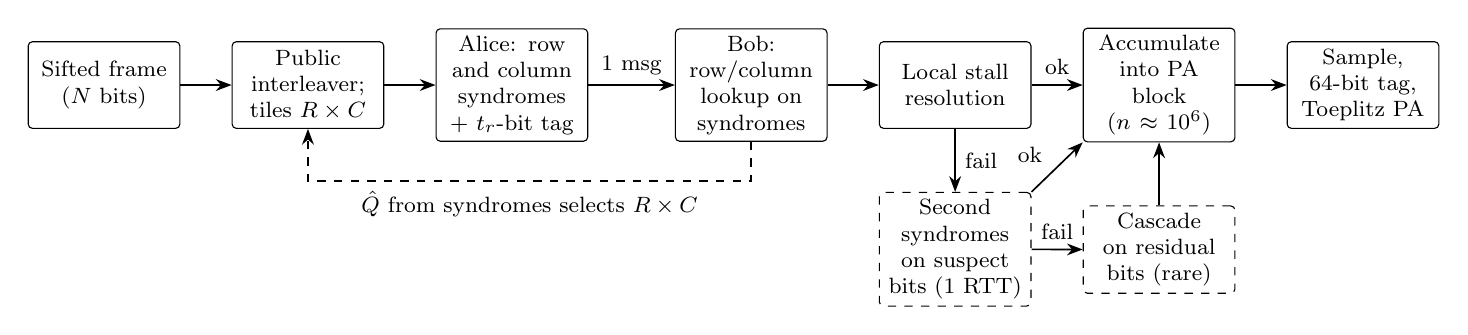
\begin{tikzpicture}[font=\footnotesize, node distance=6.5mm,
  box/.style={draw, rounded corners=1.5pt, align=center, inner sep=2.5pt, minimum height=11mm, text width=17.5mm},
  alt/.style={box, dashed},
  arr/.style={-{Stealth[length=2mm]}, semithick}]
\node[box] (s) {Sifted frame\\($N$ bits)};
\node[box, right=of s] (t) {Public interleaver;\\tiles $R\times C$};
\node[box, right=of t] (a) {Alice: row and column syndromes $+$ $t_r$-bit tag};
\node[box, right=11mm of a] (d) {Bob: row/column lookup on syndromes};
\node[box, right=of d] (st) {Local stall resolution};
\node[box, right=of st] (acc) {Accumulate into PA block ($n\approx10^6$)};
\node[box, right=of acc] (pa) {Sample, 64-bit tag, Toeplitz PA};
\node[alt, below=8mm of st] (f2) {Second syndromes on suspect bits (1 RTT)};
\node[alt, below=8mm of acc] (cas) {Cascade on residual bits (rare)};
\draw[arr] (s) -- (t);
\draw[arr] (t) -- (a);
\draw[arr] (a) -- node[above]{1 msg} (d);
\draw[arr] (d) -- (st);
\draw[arr] (st) -- node[above]{ok} (acc);
\draw[arr] (acc) -- (pa);
\draw[arr] (st) -- node[right]{fail} (f2);
\draw[arr] (f2) -- node[above]{fail} (cas);
\draw[arr] (f2.north east) -- node[above left, pos=0.4]{ok} (acc.south west);
\draw[arr] (cas) -- (acc);
\draw[arr, dashed] (d.south) -- ++(0,-5mm) -| node[pos=0.25, below]{$\hat Q$ from syndromes selects $R\times C$} (t.south);
\end{tikzpicture}
\caption{Reconciliation pipeline with LUCID-2D, the fallback ladder (dashed boxes) and block-level privacy amplification. Only the first message is needed when a frame decodes; the dashed arrow is the syndrome-based QBER estimate that selects the tile shape of the next frame.}
\label{fig:pipeline}
\end{figure*}

\section{Methodology}\label{sec:method}
\subsection{Simulator and Schemes}
A single Python simulator implements all schemes on the error pattern. \textit{Cascade} \cite{cascade} uses four passes with doubling blocks, binary search and back-tracking; all searches that can proceed in parallel do so, and one parity request--response is one round trip, so the reported rounds are a lower bound. \textit{LUCID (1-D)} uses blocks of $C\in\{8,\ldots,1024\}$ bits with the original whole-frame fallback at $N=512$ and the fallback ladder elsewhere. \textit{LUCID-2D} uses tiles with $8\le R\le C\le1024$. \textit{BP-LDPC} uses a random code with variable degree three, distinct checks per column and balanced check degrees, $m=\lceil f\,h(Q)N\rceil$ syndrome bits, and sum-product decoding \cite{kschischang2001} with up to 100 iterations; failed frames are lost. Cascade and LDPC are given the true QBER, which favours them.

\textit{Parameter selection.} For every scheme, frame size and QBER, the parameter (block size, tile shape, Cascade first block $k_1$, or $f$) is chosen on a pilot run and the reported values come from an independent run with fresh seeds. At $N=512$ the criterion is the largest $r$, as in the original study. At matched frame sizes, LUCID variants maximize $r$ subject to $\rho\le1.1$ (``one round''), or $r/\rho$ when no parameter meets this budget; Cascade maximizes $r/\rho$; and LDPC, which always needs one round, maximizes $r$. Final runs use 2000 frames at $N=512$ and 400 frames (LUCID) or 100 frames (Cascade, LDPC) at $N=16384$ and $65536$; the 95\% confidence half-width of $r$ is at most 0.011 at $N=512$ and 0.002 at $N=65536$.

\subsection{Hardware Flow}
The LUCID-2D decoder core is written in Verilog, checked cycle by cycle against a Python model of the syndrome-domain decoder with Icarus Verilog \cite{icarus} (flips, convergence, scan and cycle counts; zero mismatches over 520 random tiles of six shapes), and synthesized with Yosys and placed and routed with nextpnr \cite{shah2019}. Stall resolution and the fallback ladder are rare control paths and are not part of the core.

\section{Results}\label{sec:results}

\subsection{Validation and Reproduction}
The photon-level BB84 simulator matches $Q=e+p/4-ep/2$ to within 0.0011 at all five tested $(e,p)$ points with $3\times10^{5}$ qubits. Table~\ref{tab:repro} reproduces the original $N=512$ comparison under frame-local accounting. The secret fractions agree with the original golden model to within 0.045 and rank the three schemes identically at every QBER. At this size the one-dimensional hybrid trails Cascade in $r$, lies above the unoptimized LDPC code up to 0.5\% QBER and below it at 1\% and 2\%, and the 64-bit tag alone costs 0.125 of every key bit. Choosing the block size for throughput instead of $r$, it delivers 6.0, 5.6 and 3.1 times the round-trip-limited secret throughput of Cascade at 0.1, 0.2 and 0.5\% QBER and falls below Cascade at 2\% (0.71 times), consistent with the original study.

\begin{table}[t]
\caption{Secret Fraction $r$ and Mean Round Trips $\rho$ at $N=512$, Frame-Local Accounting (64-bit Tag per Verification)}
\label{tab:repro}
\centering
\setlength{\tabcolsep}{4pt}
\begin{tabular}{@{}lcccccc@{}}
\toprule
& \multicolumn{2}{c}{Cascade} & \multicolumn{2}{c}{LUCID (1-D)} & \multicolumn{2}{c}{BP-LDPC}\\
\cmidrule(lr){2-3}\cmidrule(lr){4-5}\cmidrule(l){6-7}
QBER (\%) & $r$ & $\rho$ & $r$ & $\rho$ & $r$ & $f$\\
\midrule
\tablerows{tables/reproduction.tex}
\bottomrule
\end{tabular}
\end{table}

\subsection{One-Round Decoding Success}
Fig.~\ref{fig:success} compares lookup-only decoding (no fallback) at equal frame size and equal row code. With 128-bit one-dimensional blocks, a 16384-bit frame decodes with probability 0.373 at 0.1\% QBER and 0.031 at 0.2\%; with 256-bit blocks, a 65536-bit frame decodes in 0.05\% of trials at 0.1\% QBER. Adding the column syndromes changes this qualitatively: with stall resolution, the $128\times128$ grid decodes every one of 2000 frames at 0.2\% and 97.7\% at 0.5\%, and the $256\times256$ grid decodes 99.6\% at 0.2\%. Stall resolution raises success where stalls dominate---from 0.894 to 0.977 for $128\times128$ at 0.5\%, and from 0.697 to 0.859 for $256\times256$ at 0.3\%---but cannot help once many lines fail, because it is limited to 16 candidate intersections. Tiles need on average 1.0--2.7 row--column iterations at QBER up to 0.2\%.

\begin{figure}[t]
\centering
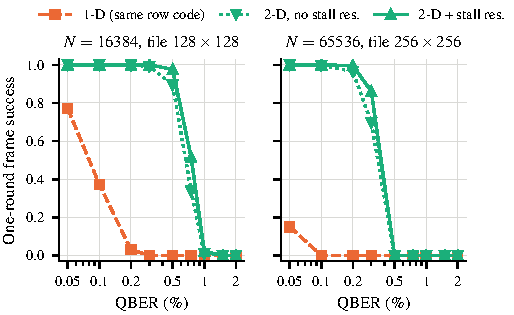
\includegraphics[width=\columnwidth]{figures/fig_success.pdf}
\caption{Probability that a frame decodes with the lookup alone (no fallback), for one-dimensional blocks and for a single square tile with the same row code.}
\label{fig:success}
\end{figure}

\subsection{Matched Frame Size}
Table~\ref{tab:matched} compares all schemes at $N=65536$ under block-level accounting, and Fig.~\ref{fig:pareto} shows the secret fraction against round trips for every configuration in a separate sweep. At 0.1\% and 0.2\% QBER the selected configuration is a single $256\times256$ tile per frame. It reaches $r=0.919$ and $0.910$, that is 96.3\% and 98.2\% of BP-LDPC ($0.954$ and $0.927$), in $\rho=1.00$ round trips. Cascade attains the highest secret fraction ($0.974$ and $0.953$) but needs 33 round trips, so when the round-trip time dominates, LUCID-2D delivers 31 times the secret throughput of Cascade. The one-dimensional lookup cannot do the same: within one round its best option at 0.2\% discloses half of the key ($r=0.478$ with 8-bit blocks), and longer blocks trigger fallbacks on most frames. At 0.5\% LUCID-2D reaches $0.813$ with $64\times256$ tiles at $\rho=1.12$ (94\% of BP-LDPC); at 1\% and 2\% it falls to 85\% and 52\% of BP-LDPC, which is then clearly preferable. Fig.~\ref{fig:pareto} shows that LUCID-2D shares the one-round corner of the trade-off only with LDPC, while Cascade and the fallback-heavy one-dimensional configurations reach comparable secret fractions only with tens to hundreds of round trips. At $N=16384$ the picture is the same, with LUCID-2D at 92.9--99.4\% of BP-LDPC up to 0.5\% QBER.

\begin{table*}[t]
\caption{Secret Fraction $r$ and Mean Round Trips $\rho$ at $N=65536$, Block-Level Accounting. LUCID Parameters Were Selected for $\rho\le1.1$ on a Pilot Run Where Possible}
\label{tab:matched}
\centering
\begin{tabular}{@{}lccccccccc@{}}
\toprule
& \multicolumn{2}{c}{Cascade} & \multicolumn{2}{c}{LUCID (1-D)} & \multicolumn{3}{c}{LUCID-2D} & \multicolumn{2}{c}{BP-LDPC ($\rho=1$)}\\
\cmidrule(lr){2-3}\cmidrule(lr){4-5}\cmidrule(lr){6-8}\cmidrule(l){9-10}
QBER (\%) & $r$ & $\rho$ & $r$ & $\rho$ & tile & $r$ & $\rho$ & $r$ & $f$\\
\midrule
\tablerows{tables/matched_N65536.tex}
\bottomrule
\end{tabular}
\end{table*}

\begin{figure}[t]
\centering
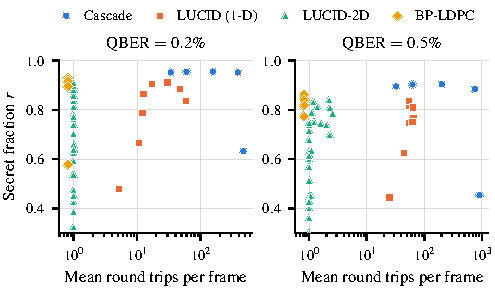
\includegraphics[width=\columnwidth]{figures/fig_pareto.pdf}
\caption{Secret fraction versus mean round trips per frame for every parameter in a sweep at $N=65536$ (block-level accounting). All LDPC points have exactly one round and are shifted left for visibility.}
\label{fig:pareto}
\end{figure}

\subsection{Ablation}
Table~\ref{tab:ablation} isolates stall resolution and the second-syndrome step. Without either mechanism a $256\times256$ tile at 0.2\% QBER falls back in 3.7\% of frames, and each fallback costs about 20 Cascade round trips ($\rho=1.76$). Stall resolution alone removes most fallbacks (0.3\%, $\rho=1.15$); the second syndrome message alone makes the remaining ones cheap ($\rho=1.03$); together they give $\rho=1.00$. At 0.5\% the two are complementary, reducing $\rho$ from 11.5 to 1.24 for $128\times128$ tiles. At 1\% with $64\times64$ tiles the second message alone is slightly better than the combination (1.85 versus 2.09), because stall-resolution guesses in tiles with many failed lines can add errors. Both mechanisms disclose so little that $r$ changes by at most 0.003.

\begin{table}[t]
\caption{Ablation at $N=65536$: Mean Round Trips $\rho$ Without and With Stall Resolution (SR) and the Second Syndrome Message (2S). The Secret Fraction $r$ (Shown for SR + 2S) Varies by at Most 0.003 Across the Four Variants}
\label{tab:ablation}
\centering
\setlength{\tabcolsep}{4pt}
\begin{tabular}{@{}llccccc@{}}
\toprule
& & & \multicolumn{4}{c}{$\rho$}\\
\cmidrule(l){4-7}
QBER (\%) & Tile & $r$ & neither & SR & 2S & SR + 2S\\
\midrule
\tablerows{tables/ablation.tex}
\bottomrule
\end{tabular}
\end{table}

\subsection{QBER Estimation and Closed-Loop Shape Selection}
Fig.~\ref{fig:estimator} compares the syndrome meter with the public sample rate of the original design, 64 sample bits per 512 key bits. Over the same observation window the syndrome meter on $128\times128$ tiles has 2.7--2.9 times lower relative error at 0.2\% QBER and 2.2--2.4 times lower at 1\%, while disclosing nothing; the sample in addition consumes one sifted bit in nine. A single 64-bit sample per 512-bit frame, as in the original design, contains no error at all in 88\% of frames at 0.2\% QBER, so it cannot steer per-frame choices. In a closed-loop run of 600 frames of 65536 bits whose QBER drifts between 0.1\% and 1\%, choosing the tile shape from the syndrome estimate gives $r=0.821$ at $\rho=1.22$, matching a controller that knows the true QBER ($0.821$, $\rho=1.17$). A sample-driven controller reaches $0.728$ because of the sacrificed bits, and a fixed shape tuned for 0.2\% needs $\rho=14.8$.

\begin{figure}[t]
\centering
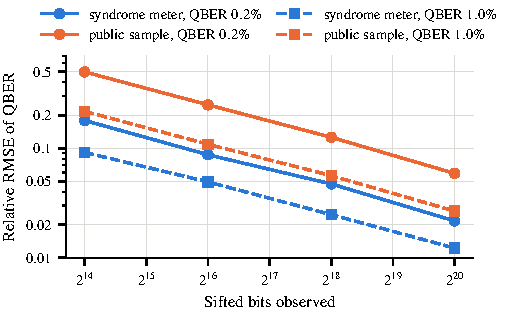
\includegraphics[width=\columnwidth]{figures/fig_estimator.pdf}
\caption{Relative root-mean-square error of the QBER estimate versus the number of sifted bits observed: syndrome meter on $128\times128$ tiles (no disclosure) and a public sample of 64 bits per 512 key bits (400 trials per point).}
\label{fig:estimator}
\end{figure}

\subsection{Finite-Key Effects}
Fig.~\ref{fig:finite} applies \eqref{eq:ell} with the leakage measured at $N=65536$, optimizing the sample size $k$ for each block size. Per-frame PA on 512 bits yields no key at any QBER (crosses). With block-level PA every scheme approaches its asymptotic value: at 0.2\% QBER and $n=2^{20}$ the finite-key fraction is 0.808 for Cascade, 0.783 for BP-LDPC and 0.767 for LUCID-2D, rising to 0.910, 0.885 and 0.868 at $n=2^{26}$. The finite-size penalty is common to all schemes, so their order is preserved; the gain over the original pipeline comes from replacing the per-frame 64-bit tag and per-frame PA.

\begin{figure}[t]
\centering
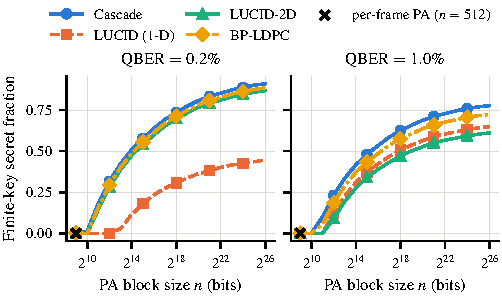
\includegraphics[width=\columnwidth]{figures/fig_finite.pdf}
\caption{Finite-key secret fraction $\ell/(n+k)$ versus PA block size, with the sample size optimized; $\varepsilon_{\mathrm{PE}}=\varepsilon_{\mathrm{PA}}=10^{-10}$. The cross marks per-frame PA of the original design.}
\label{fig:finite}
\end{figure}

\subsection{Burst Noise}\label{sec:burst}
Table~\ref{tab:burst} uses a Gilbert--Elliott channel \cite{gilbert1960,elliott1963} with no errors in the good state, error probability 0.25 in the bad state and the stationary QBER held fixed, using the tiles selected in Table~\ref{tab:matched}. When tiles are filled row by row, bursts of mean length 8 place several errors in the same row and raise the fallback rate at 0.2\% QBER from zero to 93\% ($\rho=4.25$). A fixed public pseudo-random interleaver applied before tiling spreads the bursts: the fallback rate returns to zero for $L=8$ and stays at or below 14\% at 0.2\% and 35\% at 0.5\% for $L=128$, with $\rho\le1.44$. The interleaver adds neither disclosure nor communication.

\begin{table}[t]
\caption{Fallback Rate and Mean Round Trips of LUCID-2D Under Gilbert--Elliott Noise With Mean Burst Length $L$}
\label{tab:burst}
\centering
\setlength{\tabcolsep}{4pt}
\begin{tabular}{@{}lccccc@{}}
\toprule
& & \multicolumn{2}{c}{Row-major fill} & \multicolumn{2}{c}{Interleaved fill}\\
\cmidrule(lr){3-4}\cmidrule(l){5-6}
QBER (\%) & $L$ & fallback & $\rho$ & fallback & $\rho$\\
\midrule
\tablerows{tables/burst.tex}
\bottomrule
\end{tabular}
\end{table}

\subsection{Hardware}
Table~\ref{tab:hw} lists post-route results for the decoder core on an ECP5-25F. The syndrome memories map to distributed RAM, so logic grows slowly with tile size; the $256\times256$ core selected at 0.1--0.2\% QBER uses 13.1\% of the device and closes at 61~MHz. For the AMD 7-series family, synthesis alone gives 143 logic LUTs, 48 \texttt{RAM64M} primitives and 43 flip-flops for the same core. A scan takes $R+C$ cycles; with the 2.7 iterations measured at 0.2\% QBER plus the final check, a 65536-bit tile is decoded in about 1900 cycles, 31~\textmu s at 61~MHz, or 2.1~Gbit/s of sifted key per core---less than the round-trip time of any fibre link longer than about 3~km. Computing the syndromes adds $N/W$ cycles in the front end. On an iCE40 HX8K, which has no distributed RAM, the $64\times128$ core needs 3953 logic cells at 37.8~MHz and the $256\times256$ core does not fit. By comparison, a BP decoder for the same frame stores one message per edge, $3N=196{,}608$ messages or about 1.2~Mbit at an assumed 6-bit quantization, and our BP decoder used 7--13 iterations on average, against 4.6~kbit of syndrome state and 1.1--3.9 row--column iterations for LUCID-2D.

\begin{table}[t]
\caption{LUCID-2D Decoder Core After Place and Route on a Lattice ECP5 LFE5U-25F (Yosys and nextpnr)}
\label{tab:hw}
\centering
\setlength{\tabcolsep}{4pt}
\begin{tabular}{@{}lccccc@{}}
\toprule
Tile & LUT4 & DPRAM & FF & Logic cells used & $f_{\max}$ (MHz)\\
\midrule
$64\times128$ & 562 & 48 & 38 & 864 (3.6\%) & 84.0\\
$128\times128$ & 536 & 64 & 39 & 934 (3.8\%) & 76.2\\
$256\times256$ & 2004 & 192 & 43 & 3170 (13.1\%) & 61.1\\
\bottomrule
\end{tabular}
\end{table}

\section{Discussion}\label{sec:discussion}
\textit{Where LUCID-2D fits.} In the low-QBER regime targeted by the original design (0.1--0.5\%), LUCID-2D reaches 94--98\% of the secret fraction of an oracle-tuned BP decoder within about one round trip, and 27--32 times the round-trip-limited throughput of Cascade. Its decoder is a hard-decision lookup that needs no estimate of the QBER to decode; the syndrome meter only selects the tile shape. Above about 1\% QBER the fixed disclosure of extended-Hamming components makes it uncompetitive, and LDPC or Cascade should be used.

\textit{Fairness of the comparison.} The LDPC baseline is an unoptimized random code; optimized codes reach efficiencies close to 1.1 at long frames \cite{elkouss2009,elkouss2011,mao2019} and would widen its lead, particularly above 0.5\%. On the other hand it is given the true QBER and the best syndrome length, and its decoding time is ignored. Cascade is given the true QBER and an optimized first block, and its rounds are a lower bound.

\textit{Pipeline.} The block-level pipeline helps every scheme, not only LUCID: at 0.1\% QBER Cascade rises from 0.828 at $N=512$ to 0.974 at $N=65536$, mainly because the per-frame 64-bit tag disappears. If each public message were authenticated with its own one-time-pad tag, interactive protocols would also spend key on every round trip; authenticating the transcript once per block avoids this for all schemes.

\textit{Smart grid.} Key refresh is not latency-critical, so for such links the value of LUCID-2D lies in fewer messages and a small, fixed-structure decoder at edge devices rather than in latency. An optional decode cache studied for the original front end is omitted: the lookup already completes in one cycle, and caching key-dependent blocks would keep secret material in hardware longer than necessary.

\textit{Threats to validity.} The noise models are independent flips and a synthetic burst model; the finite-key bound is simplified (A5); Cascade and LDPC compute times are ignored; the front-end RTL was characterized in simulation but not re-synthesized; stall resolution, the second syndrome step and the interleaver are not part of the RTL core. Confidence half-widths of $r$ are at most 0.002 at $N=65536$ and 0.011 at $N=512$.

\section{Limitations and Future Work}\label{sec:limits}
\begin{itemize}
\item The source is ideal (A1); a decoy-state analysis \cite{lim2014} with realistic loss and detectors is needed for deployment figures.
\item The finite-key bound is not the exact composable statement of \cite{tomamichel2012}, and the treatment of verification should follow \cite{tsurumaru2025}.
\item No power, ASIC or AMD timing results are reported, and no LDPC decoder was synthesized on the same device.
\item Future work: a composable decoy-state analysis; moving stall resolution and the interleaver into the RTL; BCH component codes or staircase arrangements \cite{smith2012} to raise efficiency above 0.5\% QBER; and an optimized quasi-cyclic LDPC baseline synthesized on the same FPGA.
\end{itemize}

\section{Conclusion}\label{sec:conclusion}
LUCID-BB84 reconciles BB84 keys with a one-way syndrome lookup and a verified fallback, and its front end verifies a 512-bit frame in 120~ns. Arranging frames as grids of extended-Hamming codes, decoding iteratively in the syndrome domain, resolving stalls locally and falling back with a single extra syndrome message turns this lookup into a one-round reconciler that reaches 94--98\% of the secret fraction of BP-LDPC at 0.1--0.5\% QBER, with 27--32 times the round-trip-limited throughput of Cascade. Moving verification and privacy amplification to blocks of about a million bits makes the finite-key rate positive and lets it approach the asymptotic rate as blocks grow, and the syndromes themselves provide a free, accurate QBER estimate. The decoder core is verified against its model and fits in 4--13\% of a 25k-LUT FPGA at 61--84~MHz. Above 1\% QBER, one-way LDPC remains the better choice.

% balance the columns of the last page
\IEEEtriggeratref{32}
\bibliographystyle{IEEEtran}
\bibliography{refs}

\end{document}
